\section{Main idea}
The principle of Mean shift is to move a "window" over the data set following the density gradient (see Figure \ref{shif}). The center of this window has to match a center of density in the dataset. At each iteration, we simply compute the gradient inside the window and then move it along this gradient. We repeat this iteration as long as the gradient norm is significant enough.\\
\begin{figure}[h!]
\fbox{
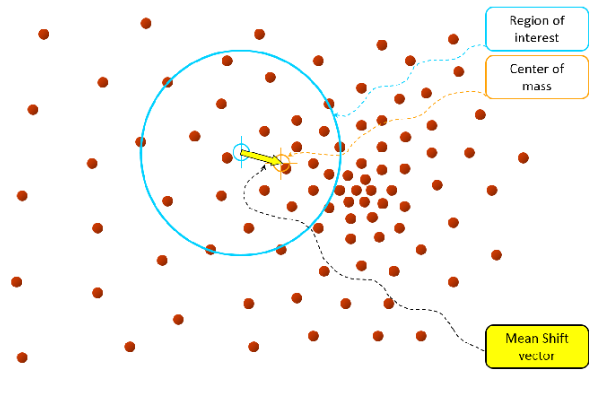
\includegraphics[width=0.32\textwidth, height=4.8cm]{Image/algo-meanshift1.png}
}
\fbox{
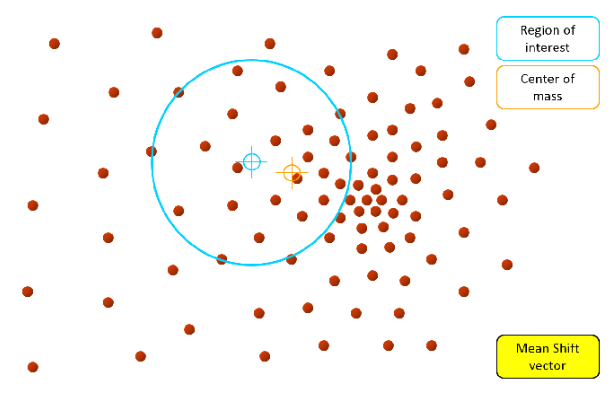
\includegraphics[width=0.32\textwidth, height=4.8cm]{Image/algo-meanshift2.png}
}
\fbox{
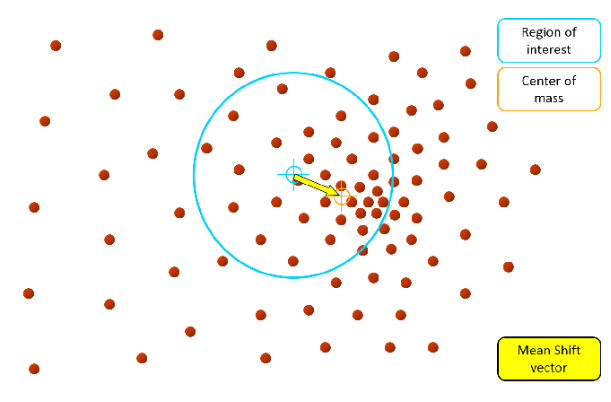
\includegraphics[width=0.32\textwidth, height=4.8cm]{Image/algo-meanshift3.png}
}
\fbox{
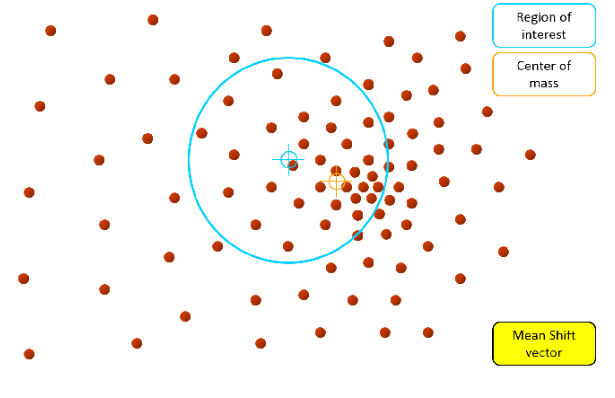
\includegraphics[width=0.32\textwidth, height=4.8cm]{Image/algo-meanshift4.png}
}
\fbox{
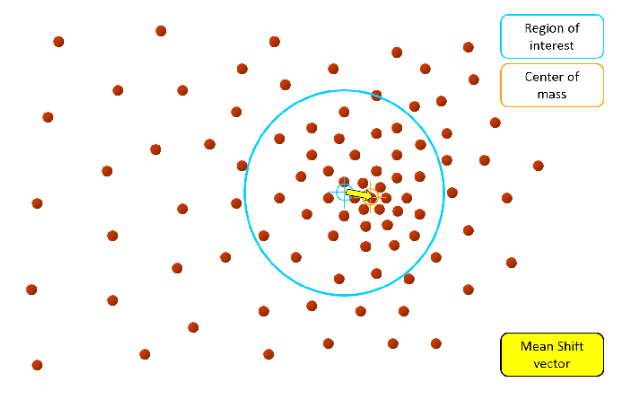
\includegraphics[width=0.32\textwidth, height=4.8cm]{Image/algo-meanshift5.png}
}
\fbox{
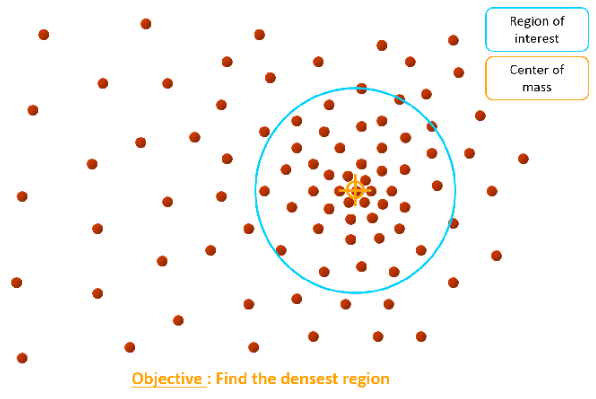
\includegraphics[width=0.32\textwidth, height=4.8cm]{Image/algo-meanshift6.png}
}
\caption{Mean shift principle\label{shif}}
\end{figure}

This simple methodology compute one cluster in the dataset. Then, we apply it again in order to cover all the points. Finally, further computations are made to merge very close clusters.

